% Document settings
\documentclass[a4paper,11pt]{article}

% Packages
  % math formulas
\usepackage{amsmath,amsthm,amssymb}
  % graphics
\usepackage{graphicx}
\usepackage{wrapfig}
  % plots
\usepackage{pgfplots}
  % other
\usepackage[warn]{mathtext}
\usepackage{cmap}
\usepackage[T1,T2A]{fontenc}
\usepackage[utf8]{inputenc}
\usepackage[english,russian]{babel}

% Package settings
%% graphicx
\graphicspath{{Pictures/}}
\DeclareGraphicsExtensions{.pdf,.png,.jpg}
%% pgfplots
\pgfplotsset{width=10cm,compat=1.9}

% Title
\title{Отчет о выполнении работы №1.3.3\\Измерение вязкости воздуха при течении в тонких трубках}
\author{Воейко Андрей Александрович, Б01-109}
\date{Долгопрудный, 2022}

% Document
\begin{document}
\maketitle
\newpage
\section{Аннотация.}
В работе определяется отношение $C_{p}/C_{v}$ для углекислого газа по ищмерению давления в стеклянном сосуде. Измерения проводятся сначала после адиабатического расширения, а затем после нагревания газа до комнатной температуры.
\section{Теоретические сведения и экспериментальная установка.}
\subsection{Экспериментальная установка.}
Используемая для опытов установка состоит из стеклянного сосуда А (см. рисунок~\ref{fig:img1}), снабженного краном К и U-образным жидкостным манометром М, измеряющим избыточное давление газа в сосуде.
\begin{wrapfigure}{r}{0.7\textwidth}
  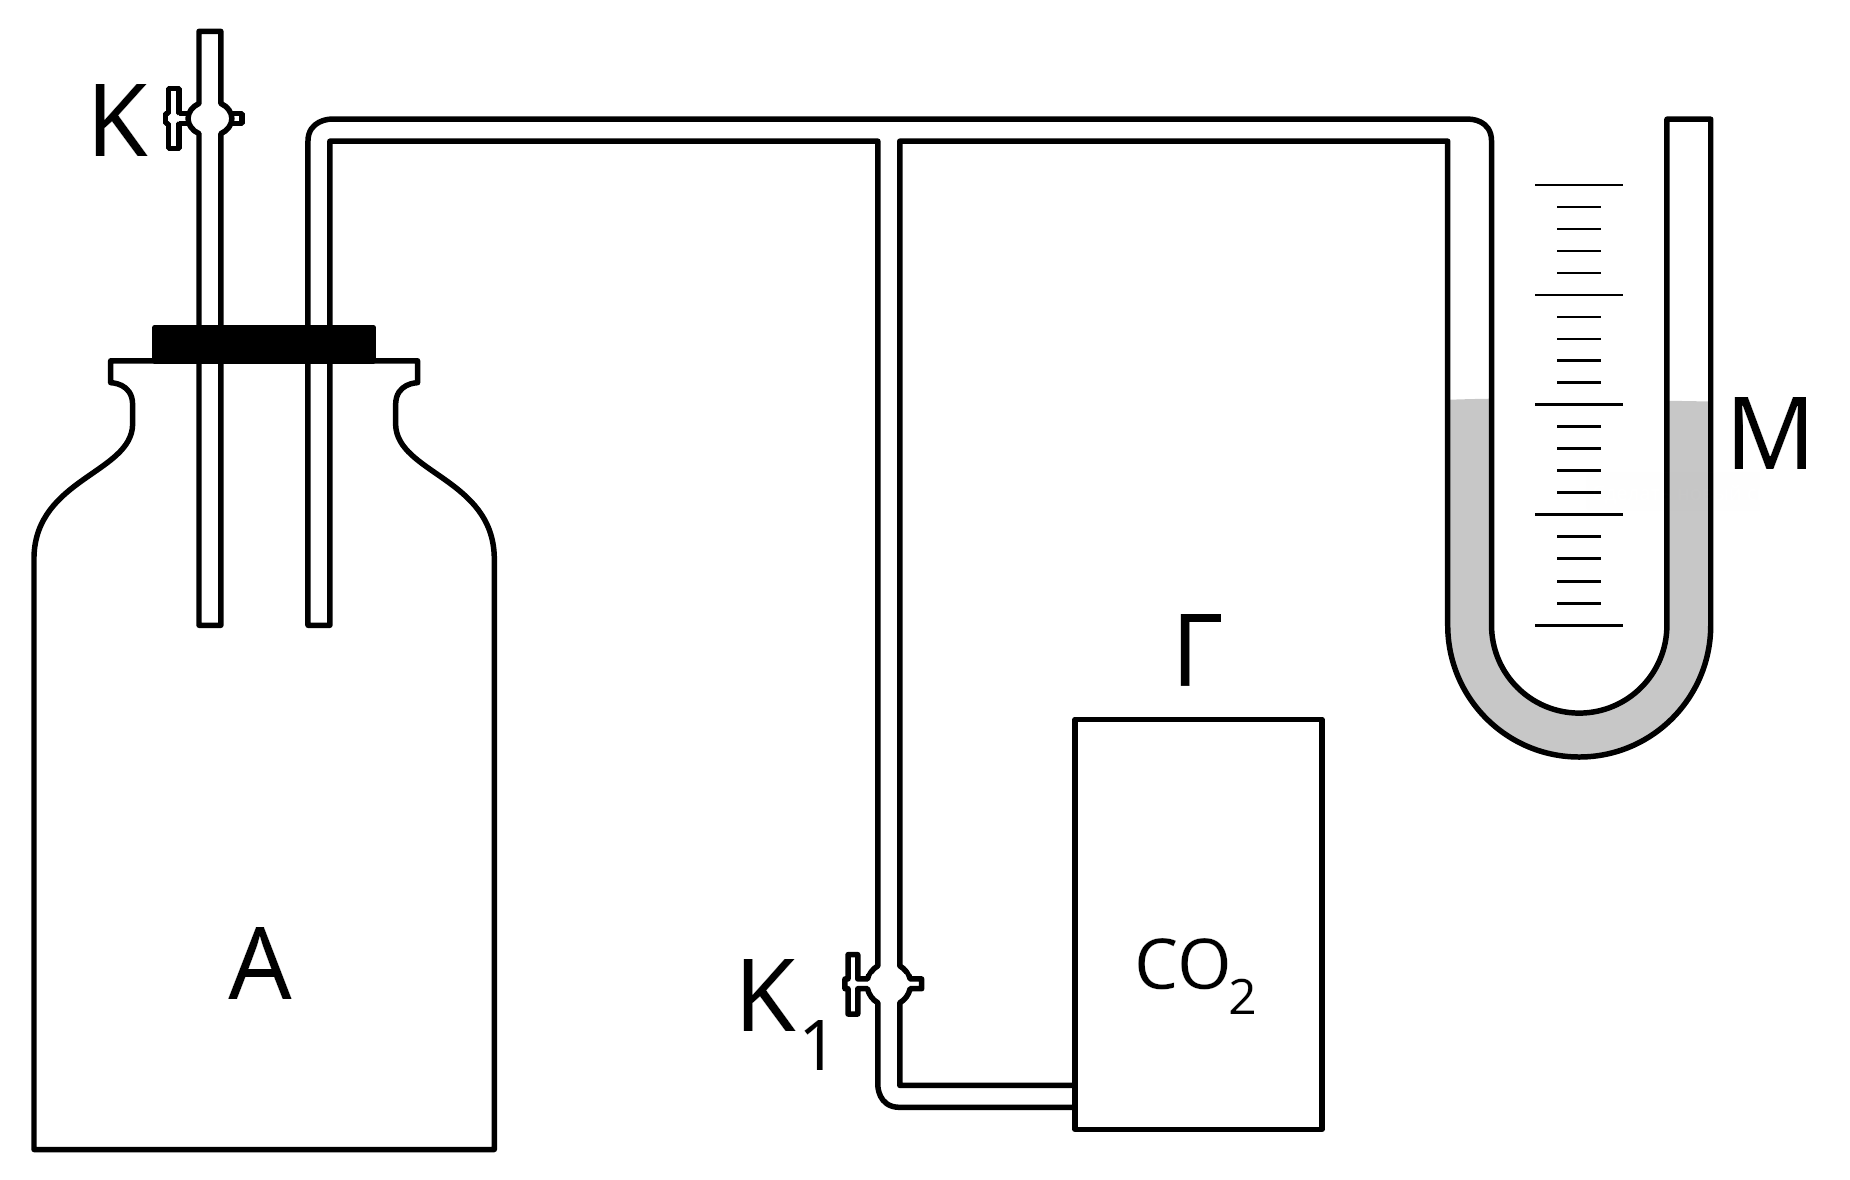
\includegraphics[scale = 0.224]{scheme1.png}
  \caption{Схема экспериментальной установки.}
  \label{fig:img1}
\end{wrapfigure}
Само избыточное давление создается путем закачивания в сосуд углекислого газа из газгольдера Г, соединенного с сосудом через кран $К_{1}$. В начале опыта в сосуде имеется газ при комнатной температуре $T_{1}$ и давлении $P_{1}$, несколько превышающем атмосферное давление $P_{0}$. После открытия крана К, соедияющего сосуд А с атмосферой, давление и температура газа будут понижаться. Это уменьшение можно считать квазиадиабатическим, так как процесс изменения давления происходит значительно быстрее изменения температуры.\\
Преобразуем уравнение адиабаты с помощью уравнения Клапейрона к переменным $P$, $T$. Обозначим состояние газа после повышения давления в сосуде и выравнивания температуры индексом <<1>>, а сразу после открытия крана и выравнивания давления с атмосферным давлением -- индексом <<2>>.\\
\begin{equation}    \label{eq1}
  \left(\frac{P_{1}}{P_{2}}\right)^{\gamma - 1} = \left(\frac{T_{1}}{T_{2}}\right)^{\gamma}.
\end{equation}
Давление $P_{2}$ после адиабатического расширения газа равно атмосферному давлению $P_{0}$, а температура $T_{2}$ будет ниже комнатной температуры $T_{1}$ (температура газа понижается, так как работа расширения совершается за свет внутренней энергии газа).\\
После того, как кран К отсоединит сосуд от атмосферы, происходит медленное изохорическое нагревание газа со скоростью, определяемой теплопроводностью стеклянных стенок сосуда. Вместе с ростом температуры растет и давление газа. За время порядка $\Delta t_{T}$ система достигает равновесия, и установившаяся температура газа $T_{3}$ становится равной комнатной $T_{1}$.\\
Изохорический процесс выравнивания температуры при закрытом кране подчиняется закону Гей-Люссака:
\begin{equation}    \label{eq2}
  \frac{P_{2}}{T_{2}} = \frac{P_{3}}{T_{3}} = \frac{P_{3}}{T_{1}}.
\end{equation}
Исключая таким образом отношение температур, получаем:
\begin{equation}    \label{eq3}
  \left(\frac{P_{3}}{P_{2}}\right)^{\gamma} = \left(\frac{P_{1}}{P_{2}}\right)^{\gamma - 1}.
\end{equation}
Отсюда:
\begin{equation}    \label{eq4}
  \gamma = \frac{ln(P_{1}/P_{0})}{ln(P_{1}/P_{3})}.
\end{equation}
Учитывая, что $P_{1} = P_{0} + \rho gh_{1}$, $P_{3} = P_{0} + \rho gh_{2}$, получаем
\begin{equation}    \label{eq5}
  \gamma = \frac{ln(1 + \rho g h_{1}/P_{0})}{ln(1 + \rho g h_{1}/P_{0}) - ln(1 + \rho g h_{2}/P_{0})} \approx \frac{h1}{h1-h2}.
\end{equation}
\subsubsection{Время протекания газа.}
Оценим время выравнивания давления $\Delta t_{p}$, пренебрегая вязкостью газа. В данном случае это можно сделать из-за малой длины трубки, через которую вытекает газ.\\
После открытия крана К по газу со скоростью звука $c$ будет распространяться волна разрежения $L/c$ (где $L$ -- высота сосуда) она достигает дна. Весь газ придет в движение, и через несколько таких интервалов процесс вытекания будет почти установившимся, квазистационарным. При этом скорость истечения $v$ можно расчитать по уравнению Бернулли для несжимаемой среды, поскольку давление воздуха мало отличается от атмосферного и изменением плотности допустимо пренебречь:
$$v = \sqrt{2(P - P_{0})/\rho_{0}\ }.$$
За время $dt$ из сосуда через отверстие площадью $S_{r}$, вытечет масса газа $\rho_{0} S_{r}vdt$, где плотность взята при атмосферном давление из-за малого изменения давления газа.\\
В сосуде объема $V_{0}$ давление за это же время снизится на $dP$, и масса газа при адиабатическом истечение уменьшится на величину
$$dm = V_{0}d\rho = \frac{V_{0}}{c^{2}}dP.$$
Здесь использовано определение адиабатической скорости звука
$$c^{2} = \left(\frac{\delta P}{\delta \rho}\right)_{S}.$$
Составив баланс вытекающей массы и остающейся в сосуде, получим диццеренциальное уравнение:
$$\frac{dP}{\sqrt{P-P_{0}\ }} = - \frac{S_{r} c^{2}\sqrt{2 \rho_{0}}}{V_{0}}dt.$$
Интегрируя, найдем искомое время вытекания газа:
\begin{equation}    \label{eq6}
  t_{P} = \frac{V_{0}}{S_{r}c} \sqrt{\frac{2(P - P_{0})}{\gamma P_{0}}\ }.
\end{equation}
Используя приблизительные данные установки, находим $t_{P} = 0,1\ с$.
\section{Результаты измерений и и обработка данных.}
\subsection{Оценка времени теплообмена $\Delta t_{T}.$}
Проведем опыт по оценке  $\Delta t_{T}$. Для этого наберем углекислого газа в сосуд и подождем, пока давление газа в сосуде перестанет меняться, следя за результатами.
% Начало таблицы 1 {{{
\begin{table}[h!]
\centering
\begin{tabular}{ ||c|c|c|c|c|| }
  \hline
  № & Прошло, $с$ & $h_{1}$, см & $h_{2}$, см & $\Delta h$, см \\
  \hline
  1 &  $60 \pm 10$ & $22,1 \pm 0,1$ & $11,4 \pm 0,1$ & $10,7 \pm 0,2$ \\
  2 & $120 \pm 10$ & $22,0 \pm 0,1$ & $11,5 \pm 0,1$ & $10,5 \pm 0,2$ \\
  3 & $240 \pm 10$ & $21,9 \pm 0,1$ & $11,6 \pm 0,1$ & $10,4 \pm 0,2$ \\
  4 & $330 \pm 10$ & $21,8 \pm 0,1$ & $11,7 \pm 0,1$ & $10,1 \pm 0,2$ \\
  5 & $480 \pm 10$ & $21,7 \pm 0,1$ & $11,7 \pm 0,1$ & $10,0 \pm 0,2$ \\
  6 & $600 \pm 10$ & $21,7 \pm 0,1$ & $11,7 \pm 0,1$ & $10,0 \pm 0,2$ \\
  \hline
\end{tabular}
\caption{Результаты измерения зависимости избыточного давления от времени.}
\label{table:tab1}
\end{table}
% }}} Конец таблицы 1
В таблице в качестве погрешности для времени указано $10\ с$, так как для нахождения высоты столбиков и разницы результатов требуется время. Тем не менее, считать это проблемой не стоит, так как вычисления носят оценочный характер.\\
На основании этих данных построим график зависимости избыточного давления от времени.
% Граф. 1 {{{
\begin{center}
\begin{tikzpicture}
\begin{axis}[
    xlabel = {$t$, $с$},
    ylabel = {$\Delta h$, $см$},
    % xmin = 25,
    % xmax = 3,
    ymin = 9,
    ymax = 12,
    grid = major,
    minor tick num = 6
]
\addplot[
    mark size=1.7pt,
    only marks,
    % only Marx,
    blue,
]
table {
    x   y
    60  10.7
    120 10.5
    240 10.3
    330 10.1
    480 10.0
    600 10.0
};
\end{axis}
\end{tikzpicture}\newline
Рис. 2: Зависимость избыточного давления от времени.
\end{center}
% }}}
Таким образом из графика видно, что 10 минут хватает для теплообмена.
\subsection{Результаты измерений.}
% Начало таблицы 2 {{{
\begin{table}[h!]
\centering
\begin{tabular}{ ||c|c|c|c|c|c|c|c|c|| }
  \hline
  & \multicolumn{3}{|c|}{До открытия крана} & \multicolumn{3}{|c|}{После открытия крана} & & \\
  \cline{2-7}
  \raisebox{1.5ex}[0cm][0cm]{№} & $h_{1}$, см & $h_{2}$, см & $\Delta h$, см & $h_{1}$, см & $h_{2}$, см & $\Delta h$, см & \raisebox{1.5ex}[0cm][0cm]{$\gamma$} & \raisebox{1.5ex}[0cm][0cm]{$\Delta t$, $с$} \\
  \hline
  & $21,7$ & $11,7$ & $10,0$ & $18,0$ & $15,4$ & $2,6$ & $1,35$ & $0,5$ \\
  \raisebox{1.5ex}[0cm][0cm]{1} & $\pm 0,1$ & $\pm 0,1$ & $\pm 0,2$ & $\pm 0,1$ & $\pm 0,1$ & $\pm 0,2$ & $\pm 0,10$ & $\pm 0,3$ \\
  & $21,8$ & $11,6$ & $10,2$ & $17,9$ & $15,5$ & $2,4$ & $1,31$ & $0,5$ \\
  \raisebox{1.5ex}[0cm][0cm]{2} & $\pm 0,1$ & $\pm 0,1$ & $\pm 0,2$ & $\pm 0,1$ & $\pm 0,1$ & $\pm 0,2$ & $\pm 0,09$ & $\pm 0,3$ \\
  & $21,5$ & $11,9$ & $9,6$ & $17,8$ & $15,6$ & $2,2$ & $1,30$ & $0,7$ \\
  \raisebox{1.5ex}[0cm][0cm]{4} & $\pm 0,1$ & $\pm 0,1$ & $\pm 0,2$ & $\pm 0,1$ & $\pm 0,1$ & $\pm 0,2$ & $\pm 0,10$ & $\pm 0,3$ \\
  & $21,3$ & $12,3$ & $9,0$ & $17,7$ & $15,7$ & $2,0$ & $1,29$ & $1,0$ \\
  \raisebox{1.5ex}[0cm][0cm]{3} & $\pm 0,1$ & $\pm 0,1$ & $\pm 0,2$ & $\pm 0,1$ & $\pm 0,1$ & $\pm 0,2$ & $\pm 0,10$ & $\pm 0,3$ \\
  & $21,4$ & $12,0$ & $9,4$ & $17,6$ & $15,8$ & $1,8$ & $1,24$ & $4,0$ \\
  \raisebox{1.5ex}[0cm][0cm]{5} & $\pm 0,1$ & $\pm 0,1$ & $\pm 0,2$ & $\pm 0,1$ & $\pm 0,1$ & $\pm 0,2$ & $\pm 0,09$ & $\pm 0,3$ \\
  & $21,3$ & $12,1$ & $9,2$ & $17,6$ & $15,8$ & $1,8$ & $1,24$ & $4,0$ \\
  \raisebox{1.5ex}[0cm][0cm]{6} & $\pm 0,1$ & $\pm 0,1$ & $\pm 0,2$ & $\pm 0,1$ & $\pm 0,1$ & $\pm 0,2$ & $\pm 0,09$ & $\pm 0,3$ \\
  & $21,2$ & $12,2$ & $9,0$ & $17,5$ & $15,9$ & $1,6$ & $1,22$ & $5,0$ \\
  \raisebox{1.5ex}[0cm][0cm]{7} & $\pm 0,1$ & $\pm 0,1$ & $\pm 0,2$ & $\pm 0,1$ & $\pm 0,1$ & $\pm 0,2$& $\pm 0,09$ & $\pm 0,3$ \\
  \hline
\end{tabular}
\caption{Результаты измерения избыточного давления до и после открытия крана.}
\label{table:tab2}
\end{table}
% }}} Конец таблицы 2
На основании этих данных построим график. Аппроксимирируем данные к прямой, $\gamma = a + b \Delta t$.
% Граф. 1 {{{
\begin{center}
\begin{tikzpicture}
\begin{axis}[
    xlabel = {$t$, $с$},
    ylabel = {$\gamma$},
    xmin = -0.2,
    xmax = 6,
    ymin = 1.19486,
    ymax = 1.4,
    grid = major,
    minor tick num = 6
]
\addplot[
    mark size=1.7pt,
    only marks,
    % only Marx,
    blue,
]
table {
    x   y
    0.5 1.35
    0.5 1.31
    0.7 1.30
    1.0 1.29
    4.0 1.24
    4.0 1.24
    5.0 1.22
};
\addplot[
    mark size=1.7pt,
    no marks,
    % only Marx,
    green,
]
table {
    x   y
    0.1 0.0
    0.1 1.45
};
\addplot[
    mark size=1.7pt,
    no marks,
    % only Marx,
    black,
]
table {
    x    y
    -0.2 1.330252
     6.0 1.194864
};
\addplot[
    mark size=2.2pt,
    only marks,
    % only Marx,
    black,
]
table {
    x   y
    0.1 1.323701
};
\end{axis}
\end{tikzpicture}\newline
Рис. 2: Зависимость избыточного давления от времени.
\end{center}
% }}}
$$b = \frac{\left<xy\right> - \left<x\right>\left<y\right>}{\left<x^{2}\right> - \left<x\right>^{2}} = -0,0218$$
$$\sigma_{b} = \frac{1}{\sqrt{7\ }}\sqrt{\frac{\left<y^{2}\right> - \left<y\right>^{2}}{\left<x^{2}\right> - \left<x\right>^{2}} - b^{2}\ } = -0,0035$$
$$a = \left<y\right> - b \left<x\right> = 1,33$$
$$\sigma_{a} = \sigma_{b}\sqrt{\left<x^{2}\right> - \left<x\right>^{2}\ } = 1,33$$
Теперь, зная эти коэффиценты, найдем $\gamma$ при $\Delta t = 0,1\ с$.
$\gamma_{0,1} = a + 0,1b = 1,32 \pm 0,21$.
\section{Выводы.}
В работе были произведены измерения избыточных давлений для различных значений времени открытия крана. По этим данным путем экстраполяции было вычислено значение $\gamma_{0,1} = 1,32$, которое мы считаем достаточным для того, чтобы установление давления практически остановилось, но недостаточным для того, чтобы теплообмен серьезно повлиял на температуру газа в сосуде. Погрешнсть составила $\pm 0,21$, или $16\%$. Табличное значение $\gamma$ для углекислого газа, как и для любого другого газа с линейной молекулой, составляет $1,4$, то есть найденное нами $\gamma$ находится в переделах погрешности. С другой стороны, сама погрешность, как уже сказано выше, составляет $16\%$.\\
На погрешность оказывают влияние как сложность измерения высоты столбиков жидкости, так и сложность измерения времени открытия крана, ведь там в качестве погрешности выступает скорость реакции человека, то есть погрешность чуть ли не одного порядка с величиной.\\
Уменьшить погрешность измерения времени довольно просто: необходимо вместо крана установить электронный клапан, управляемый простым микроконтроллером, чтобы можно было заранее установить время его открытия. Это позволит существенно снизить погрешность, так как в роли нее будет выступать время, необходимое для открытия/закрытия клапана.\\
С давлением все несколько сложнее. Для начала, предположим, что мы не хотим использовать манометры другой конструкции. Тогда, во-первых, необходимо уменьшить влияния поверхностного натяжения, чтобы верхний край столбика воды был горизонтальным. Для этого можно использовать трубки большего диаметра и/или другую, менее вязкую жидкость, для того, чтобы она меньше цеплялась за стенки трубки. Для того, чтобы получить значительный эффект от этого улучшения, необходимо использовать не сантиметровую, а миллиметровую шкалу.\\
Другим возможным решением является использование жидкости с меньшей плотностью, чтобы сами столбцы были выше. Но большинство распространенных жидкостей, плотность которых меньше, чем у воды, либо более вязкие (различные масла, глицерин, и пр.), либо гораздо интенсивнее испаряются (бензин и другие углеводороды, спирт, ацетон), что приведет к изменению состава газа, а значит повлияет на результаты эксперимента.
\end{document}
